\pagestyle{fancy}
\lhead{\sffamily OCR A-Level Computer Science}
\chead{\sffamily \thepage}
\rhead{\sffamily Jonathan Kasongo}
\lfoot{\sffamily Candidate number: N/A}
\rfoot{\sffamily Centre number: N/A}

\chapter{Analysis}

\section{Context}
\label{sec:context}

My client Axel Alabi has asked me to create an interactive
video conferencing application to allow others to view talks 
in realtime. The current solution is to use the Zoom 
video conferencing application. While it is true that the 
application is technically sound and can work fine, there is a
large number of elderly users that also try to connect to the 
conferences. These users often don't fully understand how to 
correctly use the application and then end up accidentally 
disturbing the conference/talk \footnote{From this point 
forward we will avoid using "conference/talk", and simply
replace it with "conference".}, by leaving their microphone's
on, accidentally raising their hands and having to ask Axel
for help with their various technical issues and so on and so
forth. This makes my client's job difficult since he is in 
charge of managing the Zoom call. To combat this situation 
he would like a simple and user friendly video conferencing 
application that provides the features needed for people to 
view and interact with the conferences in easily and
comfortably in real time. This includes 
features like (but not limited to) audience participation,
the ability to speak to others via one's microphone and the
ability to vote on polls. The application should be
created specifically to help elderly people have a better 
experience whilst watching any conferences, so may also
include extra accessibility features to ensure comfortable
viewing for all, irrespective of one's age and/or disabilities.

\section{Justifying a computational method}
\label{sec:computational}

The population of elderly ones in the UK has seen a 52\% 
increase in the last 40 years. This group of people includes
a large number of those who are isolated and feel a sense of 
loneliness in their lives. However through video conferencing
these ones gain the ability to socialise and interact with 
others from the comfort of their homes. This is especially 
useful as many elderly ones have limited mobility or are bed 
bound. Without regular opputunities to socialise and interact 
humans become depressed and our mental health will begin to 
decline. By developing software to enable those disabled 
people to talk to others can improve the quality of their 
mental health significantly. When people are limited by their 
disabilities or by their illnesses the oppurtunities to go and
talk to new people in real life become far and few between. For
these people real physical interactions may not be possible,
meaning that a computational solution to their problem is not
just preferred but necessary. \vspace{0.2cm}

Accessible video conferencing software is useful to young 
people aswell. People like my client also have problems with 
current systems. In order for him to carry out his job 
effectively he requires a simple and reliable computational
solution. Current systems pose a challenge for elderly people 
to use, which in turn means that my client has to spend a good
majority of his time helping people set up their webcams,
microphones or other settings. If my client instead had access
to video conferencing software that was easy for elderly people
to understand how to use comfortably his job would be 
simplified significantly, and in order to create that new 
software it is evident that a computational method can be 
used. To justify this claim we examine the average download
speeds for UK resedentials and compare it to the amount of 
download bandwidth needed to transfer clear video and audio 
for 1 second. \textit{"Average download speed of UK home 
broadband connections was 69.4 Mbit/s"} as of 2023 \cite{data}.
To compare this speed we use data from a study that took place
at the University of Chicago \textit{"On average, these
applications used about 1-2 Mbits/s of download bandwidth"}
\cite{chicago}. Even when taking the worst case of 2 Mbits/s
of download bandwidth, only $\approx 2.88\%$ of the broadband
is used. Moreover we have evidence from the previous systems 
like Zoom that were in use, that creating such an application
is definitely amenable to a computational approach.
Applications such as Zoom are able to transfer 1080p quality
video and audio data at 30 FPS with millions of users 
worldwide. These results demonstrate the validity and
feasability of a computational approach to solving this
problem. \vspace{0.2cm}

Decomposition is a computational method that involves breaking
down complex problems into multiple smaller and more 
manageable problems. Real-time video/audio feeds is the ability
for a system to take the live video and audio from a user's 
device share it to others with negligable latency. We justify
the feature of having real-time audio and video by examining 
the client's request as in \ref{sec:context}. \textit{"My 
client ... asked me to create an interactive video conferencing
platform."} Oxford Languages define a videoconference to be 
\textit{"a conference in which participants in different 
locations are able to communicate with each other in sound and
vision."} Hence in order to satisfy the client's request we 
will need to have real-time video/audio feeds. A justification
of whether or not real-time video/audio is computationally 
feasible was given in the previous paragraph.
The problem of sharing real-time audio/video feeds between
users can be decomposed into numerous sub-problems that are
easier to accomplish. For example we could break this problem
into 4 sub-problems:

\begin{enumerate}
  \item Establish a connection to the other user's computers 
  \item Ensure user has connected a suitable webcam/microphone
  \item Access the webcam/microphone using the relevant API's
  \item{Send the video/audio data to the other users in the 
        conference}
\end{enumerate}

Breaking larger problems into multiple simpler problems 
reduces the complexity of a system and promotes a  
maintainable system. Rather than trying to debug a large and
complex system, it is much easier to debug a single function 
or class
that accomplishes only 1 task. This is because the large and 
complex system may be throwing errors for a multitude of 
reasons, perhaps it could also be throwing errors because of
one mistake that was written in the code some several hundred
lines ago. With smaller and more concise code organised into
functions and similar structures, we can tell exactly where the
code is throwing an error and start working on resolving the 
issue immediately. This problem is amenable to a computational 
approach as we are able to improve the maintainability of our
codebase by applying the technique of decomposition. Moreover
decomposition allows for a much simpler approach to problem 
solving in programming. When we face a large and complicated 
task we can first decompose the problem as we did in the 
example above, and then piece together those smaller solutions
to the sub-problems, into 1 solution that achieves our intended
goal. \vspace{0.2cm}

Often once we have decomposed a problem, patterns emerge from 
the smaller decomposed problems. In recognising these patterns
we can reduce the amount of code needed to solve each 
sub-problem by placing the common operations of each 
function/class into a function/class of it's own. In order to 
ensure these repetitive actions aren't found in my code I will
employ the use of the DRY software development principle. 
That is the "\textbf{D}on't \textbf{r}epeat \textbf{y}ourself"
principle. The purpose of the DRY principle is to avoid 
writing redundant code by replacing it with abstractions. This
principle guarentees clear and concise code. One feature of 
the problem that could benefit from pattern recognition is the 
username and passcode system. A detailed justificaiton for this
feature is provided in section \ref{sec:features} under the
sub-heading \textit{Usernames and passwords to join a call}.
There are 2 cases in which we would need to check usernames
and passwords, those are when the user initially logs into 
their account and when the user enters a passcode to enter a
video conference. Instead of writing 2 seperate pieces of
code to check for the correct username and password I could
apply pattern recognition and instead implement 1 function 
called \code{Check\_User\_and\_passcode()} to be used in both 
cases. We have seen that this problem is definitely amenable 
to a computational approach, through the application of
pattern recognition to ensure clarity and conciseness in our 
codebases. \vspace{0.2cm}

As mentioned in the above paragraph abstraction is another 
computational technique that is suited to being used in my 
solution. Abstraction is the process of removing unnecessary
details, and only keeping in the parts of the solution that are
important. Abstraction could be applied to the design of the 
UI of my application. The main focus of this application should
be for it to be simple and easy to grasp as highlighted by my 
client in section \ref{sec:interview}. So in the design of my
UI I will not give the user every single piece of information
available about the call because the vast majority of that 
information will be useless to them. Furthermore it can be 
argued that the presentation of less pieces of information is
better for the user's mental health than the presentation of
large amounts of information \cite{overchoice}. When humans 
have too many options we become unable to make descisions, so
by limiting the amount of information available to the user we
allow them to focus on the few important configurations that
they should be 
in control of, in turn permitting them to give the majority of
their attention to whomever they are having a call with. This 
appropiately demonstrates the amenability of applying
abstraction in our final application. This choice will enhance
the user's experience while on our webpage and make the design
less cluttered and more aesthetically pleasing, making the 
application more desirable to use.  \\ \vspace{0.2cm}

The final computational technique is algorithmic thinking. 
Algorithmic thinking is the process of creating a finite 
sequence of steps in order to solve a given problem. Another 
one of the main objectives for the application is for it to be
accessible to all. Adding the option to have macros, 
(programmable keys that are set to perform common actions) 
can prove to be very convienient for those with limited
mobility. If the person cannot use a mouse comfortably, then 
they will have the ability to program a selected key/button to 
be able to perform pre-determined tasks like turning video
on/off and muting/unmuting the microphone. Algorithmic thinking
can be applied when implementing this feature. The task can 
be broken into a number of finite steps like so: \\

\begin{enumerate}
  \item Ask the user what button they would like to use for the macro.
  \item Update the relevant class to ensure that the action can now occur via the macro.
  \item Save this configuration onto their account through the database.
\end{enumerate}

The approach to use algorithmic thinking is justified innately
by the nature of problem-solving itself. Algorithmic thinking
is not just convienient when applied in the example of
implementing
macros, rather it is essential to the implementation of nearly
every feature that the finished system will include. Suppose 
we did not need to apply the technique of algorithmic
thinking when programming, in other words we did not require
any finite sequence of steps to solve the problem, it means 
one of two things. Either the problem needed no sequence of 
steps because it was solved instantly or that the problem
can be solved
using an infinite sequence of steps. In the first case if the
problem needed no steps to solve it, it must have been a
trivial problem. This case wouldn't apply to this application
because if it were trivial then my client Axel Alabi would 
easily program the system himself, because of his expertise in 
computer science. The second case implies that the problem will
be solved in an infinite amount of time, however our clients
do not have an infinite amount of time to wait for the 
solution to their problems, ruling out the second case 
entirely. In showing that solving problems without algorithmic
thinking is absurd we hence show that algorithmic thinking
must be used when solving problems, sufficiently justifying 
the use of algorithmic thinking as a computational method.

\section{Stakeholders}

\begin{tblr}{ll}
  \textbf{Stakeholder: } & Axel Alabi\\
  \textbf{Category: } & Client\\
\end{tblr}
\vspace{0.2cm}

\textit{Description.} %\\ \vspace{0.05cm}
Axel Alabi is a $22$ year old male, and is currently in charge 
of managing the video broadcasts for conferences. He also
works as a data analyst for a company specialising in analysing
geographical data, and has experience working in computer 
science and related fields. \vspace{0.2cm}

\textit{How will they use the solution?} % \vspace{0.05cm}
He would use the proposed solution in order to host
videoconferences. The new system would help the 
videoconferences run smoother as he wouldn't need to worry 
about spending his time in helping users solve their technical
issues, rather he will be able to focus solely on the
conference and whether or not the visuals and the audio are
clear. \vspace{0.2cm}

\textit{Why is it appropiate to their needs?} % \vspace{0.05cm}
The proposed solution would be appropiate for my client as it
would provide a smoother and simpler system in order to host 
videoconferences on. Furthermore the new system would ensure
that he no longer faces the challenges that were discussed
in \ref{sec:context}, like users leaving their microphone's.
This will no longer happen as the new system will have a 
clear and intentional design and the user won't obliviously 
have their microphone on, without being notified. This would 
improve his life greatly as he would be able to now focus 
solely on ensuring that video and audio is clear during the 
broadcast. In removing some of Axel's issues that he faces in
his job, he should become more content and calmer with his
work life, further demonstrating how this solution will be 
appropiate to his needs.

\vspace{0.2cm}

\noindent
\begin{tblr}{ll}
  \textbf{Stakeholder: } & {People aged $\sim$ 
  \hspace{-0.2cm} $50$ and over, with limited experience
  working with technology}\\
  \textbf{Category: } & Target users/audience\\
\end{tblr}
\vspace{0.2cm}

\textit{Description.}  
This group of users typically have limited experience working 
with technology, because they will have spent the majority of
their life without modern technologies. This will be my 
application's target audience, so it is important that the 
final solution is appropiate to their needs. \vspace{0.2cm}

\textit{How will they use it?}
These users will make use of the proposed solution by joining
videoconferences that they were invited to and interacting with
them in a manner that is convienient for them. They will be 
able to interact with the videoconference by raising their 
virtual hand, indicating to the speaker that they wish to talk.
The speaker can then give them permission to talk and properly
converse with their virtual audience. Moreover the solution
will also enrich their experience by providing options for
things like macros, enabling them to perform common tasks,
like muting/unmuting a microphone with a set button.
\vspace{0.2cm}

\textit{Why is it appropiate to their needs?}
The solution will benefit them greatly as they will now no 
longer have to ask for help from others to resolve issues with
their video conferencing application. Rather they will be able
to experience a simple, easy to work with and intuitive system
for their video conferencing. Moreover the users will now gain
the oppurtunity to improve their social lifes as they will be
able to chat withtheir loved ones and friends over their web 
browsers easily. Not only will the final solution make their 
lives more convinient but it will also provide the user with
the oppurtunity to improve their mental health through
socialising and engaging in conversation with others.
\cite{social}
\vspace{0.2cm}

\noindent
\begin{tblr}{ll}
  \textbf{Stakeholder: } & IT Staff\\
  \textbf{Category: } & Support/Maintainers\\
\end{tblr}
\vspace{0.2cm}

\textit{Description.}
The IT Staff would be experienced in working with technology
because of their qualifications in this field. These people 
would be expected to have a degree/diploma in computer science,
mathematics or another closely related field. They should also 
be expected to have significant experience in working in 
various programming languages. \vspace{0.2cm}

\textit{How will they use the solution?}
This group of users would be expected to be able to update and
maintain the system as required. The staff will use the
documentation provided along with the application in order to
understand what each function and class does along with it's
purpose. Furthermore the clear and readable code will enable
them to perform any necessary changes with ease, something
they could not have done previously with the off the shelf
software they had before. \vspace{0.2cm}

\textit{Why is it appropiate to their needs?}
The solution will be appropiate to their needs as they will be
able to access the source code of the final application and 
change the application to be tailored to work well for their 
specific needs. Additionally users who enquire about the 
security of their data when using the application will be able
to check how the application handles their data themselves.
This means that the IT staff will not have to be unsure about
answering user's queries, but rather they will be able to read
the source code and give an accurate response to the user every
time.

\subsection{Current system DFD diagram level 0 - Zoom}

%\vspace{0.1cm}

\begin{figure}[h]
\label{fig:dfd}
\centering
\begin{tikzpicture}

  \node[draw, rectangle, minimum width=4cm, minimum height=1cm,
	fill=lightestgray]
	(zoom) {\large Zoom};

  \node[draw, ellipse, left=3.5cm, below=2cm,
  minimum width=3cm, minimum height=1.5cm] (user) at (zoom)
    {\large User}; 

  \node[draw, ellipse, right=3.5cm, below=2cm,
  minimum width=3cm, minimum height=1.5cm] (admin) at (zoom)
    {\large Admin};

\draw[black, -{Latex[length=2.5mm]}]
	(zoom) edge["1"]  (user);

\draw[black, -{Latex[length=2.5mm]}]
	(admin) edge["3"] [bend left=0.5cm] (user);

\draw[black, -{Latex[length=2.5mm]}]
	(user) edge["2"] [bend left=0.5cm] (admin);

\draw[black, -{Latex[length=2.5mm]}]
	(admin) edge["4"]  (zoom);

\end{tikzpicture}

\caption{Zoom DFD diagram.}
\end{figure}

\textit{An explanation of the DFD is found below. The number 
closest to each edge refers to the number in the left column
of the explanation table below.} \vspace{-0.2cm}

\begin{longtblr}[
  caption={Explanation of DFD.}
]{
  colspec={lX}, hlines, row{1}={lightestgray}
}

Edge & Commentary \\

1 & {Zoom allows user to join a video conference and gives
     user live video and audio of all the other participants 
     in the meeting. User has access to a number of 
     configurations and settings after clicking on their
     profile and then on settings.} \\

2 & {If user encounters an issue they can contact the 
     admin/host of the meeting for help. User can provide the
     context or other relevant information about the issue via
     the chat box.} \\

3 & {Admin is able to read about the user's issue via the chat
     box and they can then provide a solution to the user 
     through the the chat box. Admin is also able to invite
     other users to join the video conference by sending them
     a link or a code to join.}\\

4 & {Admin can start or stop the videoconference when
     appropiate. Admin can also interact with the app in order
     to manage the video conference. They can do things like
     spotlight speakers, screenshare images/video and mute or
     kick participants.}\\
  
\end{longtblr}

\textit{Justifying the DFD.} This level 0 DFD allows me to 
preseent a broad overview of the previous system's
functionality and how it intended to work. The DFD is crucial
to ensure that my client fully understands what the previous 
system offered to the user, this information will enable me 
and my client to verify whether or not the proposed system
will be able to replace the old system by comparing the  
systems' data flow diagrams and checking if the new system is 
capable of performing all of the tasks that the old system 
was able to. Consequently user satisfaction will increase as 
they are able to quickly adapt to the new system due to it's
familiar set of features, i.e. users won't have to complain
that they cannot use the proposed system since it doesn't 
have the features that they require in a video conferencing 
system, simultaneously improving client satisfaction.

\section{Research}
\label{sec:research}

% Researched the problem in depth looking at existing solutions
% to similar problems, identifying and justifying suitable 
% approaches based on this research.

We begin our research by observing solutions to similar 
problems. Then justifications of suitable approaches are given
based on the existing solutions.

\subsection{Zoom}

\subsection*{Accessibility features}

Zoom is a popular closed-source video chat application,
developed by Zoom video communications. From their website 
\cite{zoom} they implement 5 major features to ensure that 
\textit{"Zoom is for everyone"}. 

\begin{itemize}
  \item Live transcriptions
  \item Automatic closed captioning
  \item Customisation of font sizes
  \item Keyboard shortcuts
  \item Screen reader support
\end{itemize}

Some advantages of this software include the fact that there
is a good amount of accessibility features able to help a wide
variety of people. For instance for those who have limited 
mobility keyboard shortcuts can be set up to conveniently 
perform common tasks, whilst those who have trouble hearing
well can enable closed captioning during the meeting.

\vspace{0.2cm}

However there are still a number of limitations with the way 
these features are implemented. Automatically generated 
closed captioning is unfortunately only available in english,
and may have varying levels of accuracy depending on external
factors such as background noise, speaker's clarity and 
profiency in spoken english.

\vspace{0.2cm}

Zoom proposes a solution to the problem of exculsivity when in 
the context of video conferencing applications. Instead of only
designing the application to be usable for one group of people
they aim to instead tailor it to cater towards 
\textit{everyone}. I believe that the wide range of
accessibility features is a big advantage of the system, and 
this could motivate the descision to implement a similar set
of features in my application. However while a good number of 
features is appreciable, it is also necessary to ensure that 
these features are simple to find and to use for an optimal 
user experience. This is justified by the fact that my client
is specifically requesting an application for those who aren't
comfortable with modern technology. To solve this problem I 
could perhaps implement a built-in tutorial that demonstrates 
how to use the accessibility features to teach the user how 
they can use the application to it's fullest potential.

\subsection{Skype}

\subsection*{Accessibility features}

Skype is a proprietary messaging and video chat application
developed by Skype technologies a subsidiary of Microsoft 
\cite{skype}. From Microsoft's support webpage Skype for 
Windows 8 and above has the 3 following key accessibility 
features.

\begin{itemize}
  \item Narrator screen reader
  \item High contrast colour settings
  \item Magnifier
\end{itemize}

These features have the advantage of being especially 
accessible for blind people or for those with low vision. The 
combination of high contrast colours along with a magnifier 
and/or screen reader ensures that low vision users can still 
make use of Skype, independently. Skype also doubles up to be
an instant messaging platform, permitting users to have all 
their conversations and other communications in 1 place.

\vspace{0.2cm}

Whilst the features mentioned are very beneficial for those 
with low vision, there is no true support for people who are
hard of hearing or have low mobility. This set of features is 
one-dimensional only catering to 1 group of less abled people.

\vspace{0.2cm}

Skype proposes a solution to \textit{"help people with 
disabilities navigate and control their device as well as get
better access to online content."} 
\footnote{Quote from \url{https://support.microsoft.com/en-gb/skype/what-accessibility-features-are-available-for-skype-89c34c52-f463-437a-b3be-2ea114c5de13}}
The solution from Skype allows for disabled ones especially 
those with reduced vision to benefit from Skype the most, as 
previously discussed. Whilst Skype offers a good set of
features for the disabled, the features that they mention on 
their website are all already either implemented on most 
popular operating systems, or can be installed as browser 
extensions with a few clicks. Therefore I believe that there is
insufficient justification to take the time to implement any 
of the features that Skype implements, and will not be 
implementing any of those features.

\vspace{0.2cm}

To obtain a better understanding of the nature of the problem
and what features should be implemented in the final solution,
I decided to collect some qualititative data through an 
interview with my client. This data should allow me to have an
insight into what the final solution should look like based
on my client's requirements and desires respectively.

\subsection{Interview}
\label{sec:interview}

\begin{tcolorbox}[
  boxrule=0pt, frame empty, colback=lightestgray, arc=0pt,
  breakable, colframe=white
]
  \begin{tblr}{ll}
    \textbf{Interview with Axel Alabi} & {}\\
    \textbf{Date: } \texttt{29/06/24} &
    {\hspace{-1.5cm} \textbf{Time: } \texttt{3.50pm}}
  \end{tblr}

  \vspace{0.2cm}

  \textbf{Q:} What are some of the limitations of the current
  system used for video conferencing? \vspace{0.05cm}

  \textbf{A:} It tends to be difficult for people who aren't 
  experienced with technology to properly interact in the 
  conferences. Often times participants will accidently turn 
  their microphone on or are unable to turn their microphone
  on when the speaker invites them to. \vspace{0.25cm}

  \textbf{Q:} What are some essential features that should be
  required in the final application? \vspace{0.05cm}

  \textbf{A:} Well to start the app should allow users to see 
  and hear one another in real-time, there should be a focus on
  simplicity and users should be able to raise their virtual 
  "hand" to interact with the talk. \vspace{0.25cm}

  \textbf{Q:} What are some non-essential features that would
  be desirable in the final application? \vspace{0.05cm}

  \textbf{A:} The app could perhaps provide a suite of 
  accessibility features to allow disabled ones to have a 
  comfortable viewing experience. This may include closed
  captioning, volume control and a screen reader.
  \vspace{0.25cm}

  \textbf{Q:} What operating system should the application be 
  designed for? \vspace{0.05cm}

  \textbf{A:} There is no preference for operating systems.
  \vspace{0.25cm}

  \textbf{Q:} What are the software requirements? 
  \vspace{0.05cm}

  \textbf{A:} It should be a web-based application. Any 
  suitable mainstream programming language is fine as long as 
  the code is clear enough for me and the other IT staff to 
  understand.
  \vspace{0.25cm}

  \textbf{Q:} What is your budget for the system?
  \vspace{0.05cm}

  \textbf{A:} I'd prefer the application to be completely free
  if at all possible. \vspace{0.25cm}

  \textbf{Q:} What are the security requirements?
  \vspace{0.05cm}

  \textbf{A:} There should be some form of end to end 
  encryption to ensure that hackers or others cannot access the
  video feeds. There should also be some kind of username and 
  password system in order to enter a call. Passwords should 
  also be of a good strength e.g. at least 1 symbol, capital
  and lowercase letters.
  \vspace{0.25cm}

  \textbf{Q:} How often should database backups be made?
  \vspace{0.05cm}

  \textbf{A:} They should be made every 24 hours, so that no 
  user data is lost.
  \vspace{0.25cm}


  \textbf{Q:} How will the new system benefit you? 
  \vspace{0.05cm}

  \textbf{A:} This new system will ensure that all video 
  conferences I am in charge of managing will run much 
  smoother, not only giving me more time to work on other 
  essential tasks but also providing a better viewing
  experience for all.

\end{tcolorbox}

From this interview, I can see that my client has some features
that should definitely be included in the solution: real-time 
audio and video as well as the ability to raise and lower one's
virtual hand. Furthermore I believe that security should also 
be very important when designing the final solution. This 
should be a requirement because we don't want any of our users
to have their important data stolen during their video
conference. \vspace{0.2cm}

\subsection{Further research to examine suitable approaches}
\label{sec:further}

Bearing this in mind we should also think about suitable 
approaches to implementing a system with these features. In 
order to implement the real-time video/audio I could make use
of the WebRTC API from Google, which would enable me to 
establish secure peer to peer connections from the browser. 
Not only does this approach allow us to establish audio and 
video, but it also ensures that these connections are secure 
through the use of signalling servers. Signalling servers are
servers that manage connections between peers. To understand 
signalling servers we will go through an example. Consider 2 
users, Alice and Bob that want to have a video call. Alice 
creates an offer for Bob to connect. Consequently WebRTC 
creates a session description protocol (SDP) object. The SDP 
object holds information like media types, name of the
session and the video codec being used. This data is then 
saved to a \textit{signalling} server. Bob then reads this SDP
offer from the server and WebRTC creates a SDP answer and
writes this to the server. Alice and Bob have now established 
a peer to peer connection. In essence, signalling allows for 
users to exchange the metadata of their connection through the
WebRTC API. To justify usage of the WebRTC API, I believe it 
is first necessary to explain why I rejected the idea of
implementing an API from scratch. Unfortunately
implementations of fully functioning and secure peer to peer
API's aren't trivial at all. The time it would take to fully
understand how to implement peer to peer connections using 
VP9 packetizers \cite{vp9} and SHA-256 cryptography for data
security would simply be too time-consuming and cannot be
justified when fully functioning, tested and performant 
implementations already exist. The next 
portion of the justification covers why did I choose the
WebRTC API over other API's? WebRTC is from Google and it is 
well known that Google is a credible technology company. 
Therefore it is sensible to assume that their API is of 
highest quality publicly available right now. However, there
are alternatives to WebRTC like: VideoSDK, Twilio and 
MirrorFly. Whilst it can be acknowledged that these API's could
potentially be a better fit for my project in terms of
performance, features and simplicity, all of these alternatives
are paid for. I don't think it would be sensible to pay for
commercial API's when there are free one's like WebRTC
available that will work just fine. This reasoning is also in 
harmony with my client's request to have the application
\textit{"be completely free if at all possible."} as seen in 
the interview. \\ \vspace{0.2cm}

When discussing security it is also important to discuss the 
username and password management system that may be implemented
since it is one of my client's requests. In order to design a 
system that has secure password management it will be 
beneficial to study how other industry applications have chosen
to solve the problem of managing user passwords. I chose to 
study Bitwarden, a freemium open source password management 
service. The following information was found on their 
architecture webpage \cite{Bitwarden}. As per their website 
they use the \textit{"Command and Query Responsibility 
Segregation (CQRS) pattern"}. The CQRS model developed by 
Microsoft separates reads and writes into different models. 
\textit{Commands} are used to write to the database, whilst 
\textit{queries} are used to read from the database. Each 
command and query has one \emph{single} responsibility and 
should be based on actions rather than operations on data. For
instance Microsoft give the example rather than use the
data-based command: \code{SET ReservationStatus to Reserved}
we should prefer to use the action-based command: \\
\code{Book\_Hotel\_Room()} instead. Some of the benefits of 
this model include: 

\begin{itemize}
  \item Security. It's easier to ensure that only people of authority are performing reads and writes to the database if 
they're separated.

  \item Separation of concerns. Splitting the read and write components makes the system more modular and more maintainable. 

  \item Simplified commands. Instead of directly manipulating data commands should be based on the task they try to 
achieve.
\end{itemize}

Bitwarden's servers use the MSSQL database and makes automated
nightly backups to ensure data is protected. Nightly backups 
are backups that occur every 24 hours. Moreover the 
company uses \textit{zero-knowledge encryption} so that the 
company cannot see it's users data. To ensure zero-knowledge 
encryption the compnay uses \textit{"AES-CBC 256 bit 
encryption for the data encryption and PBKDF2 SHA-256 to 
derive one's encryption key."} \footnote{Source: 
\url{https://bitwarden.com/help/what-encryption-is-used/}} 
Through this kind of encryption the company is able to have
it's users complete trust as they are sure that their data is 
safe and cannot be read by anyone other than them. Both of 
these algorithms require large amounts of higher mathematics
in order to implement them. Fortunately
for our case we will not have to consider implementing these
algotrithms because WebRTC provides built-in encryption. \\
\vspace{0.2cm}

For this application's database we need a system that satifies
the following 2 requirements. Firstly the system must be 
cloud-based, this is because neither me or my client have 
servers available for use in this application. Secondly the 
system must be free \textit{"if at all possible"}. It turns 
out that free database hosting systems do exist provided some 
conditions, like storage limits are imposed. The following 
table details the results from some of my independent research
on this topic. \footnote{Source:
\url{https://gist.github.com/bmaupin/0ce79806467804fdbbf8761970511b8c}, Information here was personally fact-checked.}


\begin{longtblr}[
  caption={Potential database hosting systems.}
]{
  colspec={lllX}, row{1}={lightestgray}
}
  \hline
  Service & Type & Storage & Limitations\\  
  \hline

  Clever Cloud & PostgreSQL & 256 MiB & {Maximum of 5 database
  connections.}\\

  MongoDB Atlas & MongoDB & 512 MB & {N/A}\\

  Fly.io & PostgreSQL & 3 GB & {Credit card required, No way
  to avoid accidental overage fees.}\\

  Oracle Cloud & Oracle & 20 GB & {Payment method required.}\\
  
  IBM Cloudant & Propietary & 1 GB & {Data deleted after 30 
  days of no activity.}\\

  \hline
\end{longtblr}

Fly.io provides "free" database hosting on the premise that
you have to give your credit card information. Then once 
your database uses a certain amount of storage the company
automatically charges you based on the amount you used. For
this reason I feel that it is justified to rule out the
option of using Fly.io completely. If the application were
to suddenly grow to have a large userbase the database could
start charging me or my client whilst we weren't aware, this
kind of mistake could be economically catastophic for either 
one of us. IBM Cloudant delete data after 30 days of 
inactivity, meaning that large amounts of user data could 
be lost. Users should be able to use our application knowing
that their data is safe and secure, if we chose to use IBM
Cloudant then we wouldn't be able to make this guarentee. If
users lose their data it may lead to complaints and 
frustrations with the design of the new system, leading to 
poor client satisfaction and users returning to the old 
videoconferencing system. Hence I feel that it is justified 
to rule out the use of IBM Cloudant aswell. The remaining 3 
options all have their relevant advantages and no very
significant disadvantages so all 3 of them could potentially
be used in this application. \\ \vspace{0.2cm}

Another concern pertaining to passwords is our method for 
checking a potential password's strength. I propose the usage
of the \texttt{zxcvbn} algorithm \cite{pass} developed by
Dropbox. This algorithm has been implemented into a number of
programming languages by the author Daniel Wheeler, so we will
simply import one of his implementations into our codebase as
a module ensuring that only accurate and tested code is used 
in the system. To justify usage of the algorithm we should
first \textit{briefly} examine exactly what the algorithm is
doing. \footnote{Note that Daniel Wheeler explains his
algorithm at a much more in-depth level in his paper, which
may be found in the citation above, if you wish to learn
more.} \texttt{zxcvbn} consists of 3 main phases: 1) matching,
2) estimation and 3) search. Throughout the rest of this
paragraph define $p$ to be some arbitrary password of length
$n$ characters. The matching phase takes contiguous
substrings of the input password and classifies
each substring as a specific pattern like a \textit{token},
\textit{date} or a \textit{repeat}. Wheeler provides the
following example in his paper; the password
\texttt{lenovo1111} will be pattern matched like so.

\[
  \underbrace{ \mathtt{lenovo} }_\text{token} \; \;
  \underbrace{ \mathtt{1111} }_\text{repeat}
\]

Different methods are used to find each class of pattern, for 
instance in order to match tokens the algorithm first takes
a password $p$ it entirely lowercase, it then checks all 
$n(n+1)/2$ non-empty substrings with a frequency ranked
dictionary, if there are symbols in $p$ it creates extra 
strings making leet substitutions \footnote{Leet substutions are symbols that are used to replace characters like the word
\texttt{@pp1e} $\rightarrow$ \texttt{apple}.}
and does the same check on these. The next phase is
estimation where we estimate the number of guesses in order
to successfully guess each match in some password. Again
for the sake of brevity we will only consider the method to 
estimate guesses for one class of pattern: \textit{bruteforce}
patterns. \textit{Bruteforce} patterns are "patterns" with no
obvious pattern and are a random string of characters like
\texttt{ae\#U*\$gmi}. The algorithm assumes that each
character will take $C := 10$ attempts to guess correctly and 
subsequently estimates $C^n$ guesses to be required to guess
the entire substring. Finally for the last phase, we define a
match-sequence to be a sequence $s_1, s_2, ...$ of matches, 
such that no matches intersect with one another and the
matches contigously cover the \textit{entirety} of $p$. 
The search looks
for an optimal match-sequence $s_1, s_2, ...$ of length
$\left|s\right|$, from a set $S$ of all the match-sequences
found in $p$ such that this sequence $s$ has a minimal number
of guesses $m_G$ over all matches $m$ in the sequence, where 
$m_G$ is the estimated number of guesses for an attacker to 
successfully guess match $m$. More formally the algorithm 
computes;

\[
  \argmin_{s \subseteq S} \left( D^{\left|s\right| -1} + 
  \left|s\right|! \prod_{m \in s} m_G \right)
\]

using a dynamic programming algorithm,
where $D$ is a real constant that acts to bias against long
sequences that unintentionally minimise the 
$\prod_{m \in s} m_G$ term. Moreover the module provides other
information about a given password in an object 
\texttt{result}. For instance 
\texttt{result.feedback.suggestions} provides a list of 
suggestions that the user can implement in order to make their
password stronger; e.g. \textit{"Add another word or two.
Uncommon words are better."} Having now seen how the 
algorithm works the advantages of using this model are clearly
numerous. It employs the use of
rigorous and accurate mathematical models in order to estimate
the number of attempts that a password can be guessed in and 
therefore the strength of any given password in 
\emph{milliseconds}. Additionally there is built-in help for 
the user as they can consult the warnings and suggestions 
provided by the \texttt{zxcvbn} module to ensure that their
password isn't weak. \\ \vspace{0.2cm}

In September 2016 a fleet of distributed denial of service 
attacks (DDoS) were launched on multiple company's websites 
some of which exceeded 600 Gbps making it one of the largest 
DDoS attacks ever recorded \cite{mirai}. Moreover one of the 
affected companies \textit{Dyn} happened to be a major DNS
server provider; what ensued were a series of disruptions to 
some of the world's most prominent companies like Amazon, 
Twitter and Netflix. This event caused significant economic 
damage to the companies involved as well as causing harm to 
these companies public reputations. The source of the attack:
The \textit{Mirai} botnet. A botnet is a collection of 
devices with internet access, that are infected with a malware
that enables a hacker or malicious internet user to coordinate
and control the actions of the complete collection of devices
via the internet. If our web-app is attacked by a botnet 
there will be severe reprecussions for me and my client, so 
it is important to try and prevent any such occurrence before
it actually takes place. If we are to prevent bots from 
accessing our web-app we have to first deduce whether the user
is a human or a bot. This is where \textit{Completely
Automated Public Turing test to tell Computers and Humans
Apart (CAPTCHA)} comes in. CAPTCHAs aim to determine whether
or not a user is human by providing a test that only humans 
can pass. A clasical example is distorted character 
recognition,

\begin{figure}[h]
  \centering
  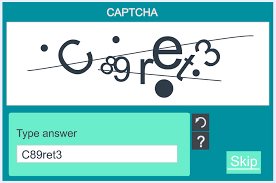
\includegraphics[scale=0.75]{Images/Captcha.png}
  \caption{A classic CAPTCHA example.}
\end{figure}

the user is presented with some jumbled and warped text and is
asked to type out the characters they see. This task used to 
be extremely difficult for computer programs to solve since 
they aren't able truly "read" these twisted characters, rather
all the computer sees is a string of \texttt{0}'s and
\texttt{1}'s that represent the given image. Nevertheless, 
computer scientists have found ways to solve these kinds of 
tasks with nearly perfect accuracy, through techniques in 
machine learning. To combat this new technology modern CAPTCHA
systems use different tests; one example is the simple 
checkbox CAPTCHA. This CAPTCHA analyses the movement of the 
user's cursor as they come to check the box. When humans move 
their cursor around a screen there is often some unintentional
random movement, that is no human can move their cursor in a 
completely straight line 100\% of the time. If the user moves 
their mouse in a completely straight line towards the
check-box then it is most likely that this user is a bot. In 
order to implement the CAPTCHA I propose the usage of the 
Altcha API. We now provide a justification for the usage of
the Altcha API. Altcha is a completely free and open source
CAPTCHA alternative. Moreover Altcha is completely GDPR 
compliant and is completely self-hosted. There are 2 main 
competitors in the market of CAPTCHA: Google's reCAPTCHA and
Cloudflare's turnstile. The main disadvantage with both of 
these systems is that they are both cloud hosted, hence both 
options impose limits on the amounts of CAPTCHA verifications 
that one can use on their website. Google permits
10,000 CAPTCHA verifications for free per month, whilst
Cloudflare offers 10 CAPTCHA widgets at most 10 different 
website hostnames. Whilst it is true that these free limits 
are generous my final descision is motivated by my client's 
words in our interview, \textit{I'd prefer the application to
be completely free if at all possible.} Altcha is completely
free and poses no limitations or restrictions on it's use 
because it is self-hosted and this API aligns itself fully 
with the requests of my client.

\subsubsection{Conclusions}

\textit{What are suitable approaches based on this research?}
The features that Zoom provides like keyboard shortcuts and 
custom font sizes would be suitable because they would aid the
user and allow them to have a more comfortable tailored 
viewing experience. The interview also provided some valuable 
information for essential features in the system, like the 
focus on simplicity. This information guides the approach to 
the design of the system, the design should be created to 
prioritse ease of use and simplicity. Moreover we have seen 
that using the WebRTC API for peer to peer video connections
is a suitable approach because of it's security, credibility
and it's alignment with the client's goal to have the system
be free if possible. Additionally we also outlined an 
approach to reading/writing to databases, the 
CQRS model. Usage of this model will help streamline the 
database for this system, because each command/query will be
clearly named and let the developer know exactly what 
processes are taking place at that moment. We selected
the \texttt{zxcvbn} algorithm to verify password strength, 
because of it's speed, accuracy and it's ability to guide the 
user into selecting a strong password through the built-in 
suggestions. Finally we chose the Altcha CAPTCHA system in 
order to prevent bot attacks on our website because it is 
fully compliant with GDPR, self-hosted and most importantly 
completely free.

\section{Essential features \& their justifications}
\label{sec:features}

\textbf{1 - Real-time audio/video feeds} \\ \vspace{0.1cm}

\textit{Explanation:} This will enable multiple users to 
connect to each other via their browsers and view each 
other's webcams, as well as hear
each other in real-time. \vspace{0.1cm}

\textit{Justification:} The justification for this feature is
that it is explicitly requested for by my client in our
interview, furthermore we don't have a \textit{video}
conferencing application if we cannot actually see other 
people's video feeds on our application. Therefore real-time
audio and video feeds are necessary for the system to perform
it's primary task.

\vspace{0.2cm}

\textbf{2 - Raising one's virtual hand} \\ \vspace{0.1cm}

\textit{Explanation:} This feature will allow people to be
able to interact with the
person giving the talk as if they were present in real life.
The virtual hand will be made visible to all participants in 
the conference so that the speaker/host will be able to ask 
the audience members to speak when appropiate.\\
\vspace{0.1cm}

\textit{Justification:} This feature
is sufficiently justified because of my client's specific 
request to implement it as a feature in the interview. 
Furthermore the implementation of this feature will help the 
migration from Zoom to our new platform be familiar as this 
feature is also found on Zoom. In a lot of talks the speaker
will sometimes ask the audience a question or ask the audience
to raise their hands in order to engage the audience with the
talk. Through the implementation of this feature we enable 
those who are attending via video conference the opportunity
to be able to engage with the speaker even though they aren't
physically present.

\vspace{0.2cm}

\textbf{3 - Designation of a host} \\ \vspace{0.1cm}

\textit{Explanation:} This feature will allow the creator of
the conference to assign 1 or multiple people to be the 
\textit{host} of the conference. That means that these
people will be in charge of 
managing the conference and will control who to admit into the
conference call, who to unmute and who to remove from the
call,and will be able to lower other's virtual hand. 
\vspace{0.1cm}

\textit{Justification:} The
justification of this feature is that I believe there should 
always be someone of some sort of authority to coordinate and 
manage these conferences. This is very common in real life
also because without management and coordination people
would be clueless, and anarchy would run rampant. This
phenomenon has been seen to occur in other video chat 
applications more specifically, on Zoom 
(e.g. See Zoombombing), and in order to provide the 
best experience for our users it is vital that events like 
this aren't allowed to occur. Through ensuring that there are
measures in place to prevent strangers from entering the
user's video call, users can be sure that their video call is
totally protected and that their privacy is maintained.

\vspace{0.2cm}

\textbf{4 - Usernames and passwords to join a call} \\ 
\vspace{0.1cm}

\textit{Explanation:} Each user will be able to choose their unique username so 
that users can easily identify one another upon joining a 
call. Furthermore each user can set their own password so 
that their account is protected and others cannot pretend to 
be them. 
Assigned to each user account will be their saved settings and
options, so that if a user has a specific configuration of 
settings that are adapted for their needs they don't have to 
set these up each time they log onto a conference. Passwords 
will be made to fit some set of requirements to ensure that 
the password is of sufficient strength. When a user creates a 
call they will be given a unique passcode that they will be 
able to share with anyone else whom they would like to invite
to the video conference. \vspace{0.1cm}

\textit{Justification:} The justification of this feature is
clearly sufficient because it was explicitly requested during
my interview with the client. Moreover without a passcode 
system to enter a call anyone would be able to enter anyone
else's call, giving users no privacy at all. It would also 
cause issues very similar to the "anarchy" problems that 
were discussed in the previous paragraph.

\vspace{0.2cm}

\textbf{5 - Simple and user friendly UI} \\ \vspace{0.1cm}

\textit{Explanation:} 
The UI should be designed in such a way that anyone could be 
able to understand how to use the application. That is the UI
should be made to be clear, intuitive and easy to navigate.
\vspace{0.1cm}

\textit{Justification:} 
This feature
aligns with the idea to have the system be accessible,
through ensuring that all users are able to navigate the 
interface without having to ask others for help. Furthermore
a nice and user-friendly interface makes the app more 
pleasant to use and the user will only have essential 
information on their screens
to make sure that the interface is not cluttered or 
overcrowded. The justification of this feature is then 
reinforced by the fact that my client requested this as an 
"essential" feature during our interview
in section \ref{sec:research}. \vspace{0.2cm}

\textbf{6 - Text-chat box} \\ \vspace{0.1cm}

\textit{Explanation:}
Users should be able to communicate with each other via text
as well as face to face through the application. On every
video conference there will be a text chat box available for
every particpant to use. \vspace{0.1cm}

\textit{Justification:}
In the potential situation that a user
lacks a microphone or forgets to turn on their microphone other 
users will still be able to communicate with them through the 
built-in chat box. This feature falls in harmony with one of 
the primary motivations for this application, that is, to have 
the system be accessible to everyone. Even if a user doesn't
have the required financial situation to be able to afford a 
microphone, they are not isolated from others, and can still 
make use of the system to talk to their colleagues, friends
or loved ones.

\section{Limitations}

\textbf{1 - Internet} \\ \vspace{0.1cm} 

\textit{Explanation:}
The application will require an internet connection. Since the
application makes use of the WebRTC API, we require internet 
access in order to establish any peer to peer connections.
\vspace{0.1cm}

\textit{Justification:}
Though accessibility is one of the main focuses of the system,
this limitation actively makes the app less accessible. This
is because people may not always have access to the internet 
whether it be due to economic, geographical or other reasons.
Hence in using the WebRTC API we have limited the number of 
potential users for our application as not everyone has 
constant access to the internet. More precisely, only 66\% of 
people have internet access in the world according to Statista.
\footnote{Source: \url{https://www.statista.com/statistics/325706/global-internet-user-penetration/}}
This limitation is sufficiently justified through the fact that
we aim to have the app be as accessible as possible, but in 
order for the application to function an internet connection is
required, hence alienating 34\% of the world's population as they
will be completely unable to use the system. \\ \vspace{0.2cm}

\textbf{2 - Passwords} \\ \vspace{0.1cm}

\textit{Explanation:}
As specified in the essential features, each user will have to 
create an account with a set username and password in order to 
use the application. \vspace{0.1cm}

\textit{Justification:} This means users will have to remember 
their passwords which could be difficult for this application's
target demographic. This means that the app will be
potentially inaccessible for people suffering from conditions
like amnesia or dementia, further restricting our possible 
userbase. If a user has forgotten their password they
may be forced to create a new account, which is a pain for the 
user as they would have to use a new username and notify all of
their contacts that their username has changed. It would also 
be a pain for the database as each time someone forgets their 
password a redundant account is left in the database, 
increasing the size of the database exponentially, if a user 
forgets their password multiple times. This limitation is 
justified by the fact that if this limitation is left to be
there will be consequences to both the user and also to the 
database. \\ \vspace{0.2cm}

\textbf{3 - Signalling servers} \\ \vspace{0.1cm}

\textit{Explanation:}
In order to use the WebRTC API for peer to peer connections we
will have to set up a signalling server as explained in 
section \ref{sec:further}. \vspace{0.1cm}

\textit{Justification:}
Signalling servers aren't
available free of charge, for example Google Firebase charges
nothing for the 
first 360MB of data transfer per day and after this they charge
\$0.15 per GB. From my interview with the client I know that 
Axel would like the system to be \textit{"completely free if
at all possible."} Whilst the prices from Firebase aren't 
extortionate by any means, the reality that my client would
prefer the application to be free means that the scalabilty of
the system would be limited. After a certain amount of data is 
transfered via the signalling server the system would no longer
work meaning the number of users we could potentially have is 
capped. To justify this being a limitation we can notice 
the fact that we require a signalling server in order to
establish a network connection means that one of the client's
requests could perhaps, not be reasonably achieved. \\
\vspace{0.2cm}

\textbf{4 - Social engineering} \\ \vspace{0.1cm}

\textit{Explanation:}
Users must have access to a computer or some other device that
allows them to connect to the internet and access websites. 
Consequently if the user logs into their account on a public 
computer they may be susceptible to various forms of social 
engineering, for example someone may be shoulder surfing the 
user whilst they are typing in their password. \vspace{0.1cm}

\textit{Justification:}
These kinds of issues may lead to a breach of data protection
regulations and users having their private information stolen.
Since we would like to maximise users' privacy we should aim 
to ensure that no strangers are able to get access to accounts
that do not belong to them. Unfortunately when dealing with 
social engineering it is not trivial for the software 
developers to completely prevent these kinds of data breaches.
To illustrate say that in order to prevent an attacker from 
viewing a user's password whilst they are typing it, the 
developer makes the password "invisisble" such that it looks
like this  $\bullet \bullet \bullet \bullet \bullet$ whilst
they are typing. An attacker knowing this could then install 
a keylogger on the computer that our user is logging onto and
will then be able to retrieve the password later.

\section{Client requirements}
% specify
%justify why they are important

\subsection{Data capture}

A microphone and video camera will be used in order to get 
video and audio footage from each user. This will enable the 
users to communicate with one another and will allow my client
to be able to host video conferences on the system. 
Justification for audio and video were provided in 
\ref{sec:computational}, so here we will justify the use of 
cameras and microphones. The approach of using microphones and
webcams to capture video and audio is fully justified by the
fact that there exists no suitable alternatives to these 
technologies. For video the only other known alternative to a
camera is to use a photogram. A photogram is a black and white
image \textit{"made by placing objects between a light 
sensitive paper or film and light source."} \cite{photo}. This
is unsuitable for video as if we want to achieve a standard
frame rate of 30 FPS the users would have to buy a large
quantity of photographic paper, costing the user a lot of
money. Furthermore photograms take roughly 1 minute to
develop, this means that the user would have to properly setup,
develop and share photograms with others at a rate of 30 times
per second, whilst waiting 1 minute for each photogram to
develop. These reasons provide sufficient justification as for
why cameras are the only suitable option. As for audio my 
independent research on this topic indicated that we have not
yet found alternatives to microphones for capturing sound. 

\subsection{Data verification and validation}

In this system data will be verified upon the creation of a
new account. Users will prompted to enter their desired
password twice in order to ensure that the user would really 
like this to be their password and that they have spelt it 
correctly. Moreover these passwords will be checked to 
ensure that they are of suitable strength. Justification for 
this feature was provided in \ref{sec:features} under 
\textit{Usernames and passwords to join a call} and a
potential implementation was discussed in \ref{sec:research}.
Data will also have to be verified before it is put into the 
database. We should ensure that all data that is being entered
into the database is of the correct data type and that
\texttt{NULL} values aren't permitted if a particular 
attribute is mandatory. The verification of data entering our
database is justified because it prevents a host of problems 
arising later on in the development of the system. For example
if we don't verify that the data in the username column is 
only of the string data type, it could be possible that 
someone's username is a \texttt{NULL} field. In this case we 
will never be able to log this user in because their account
isn't accessed by their username meaning that we will never be
able to verify that the password that they have inputted is the 
correct password that is stored in the database.

\subsection{Data processing}

In order to send video and audio data to others quickly the 
system will have to compress both. This will be managed by the
video/audio codecs that we choose to use in the beginning of
the peer to peer connection. This is handled by the
WebRTC API. Audio and video compression is 
important because without it we would have to send large 
amounts of data to others over the internet by splitting the
data up into a number of packets. Each frame would take a 
considerable amount of time to arrive completely and the user
would be presented with a slow and laggy experience.
Furthermore the more data that we have to send per second 
means that the user will require more bandwidth, and this 
may not be economically possible for all users. If we wish 
for our application to be accessible than we should develop it
in such a way that there are minimal requirements to use the 
application smoothly and compression will certainly reduce the
system requirements needed to run this application.

\subsection{Outputs}

Outputs like the video and audio from other participants will 
be displayed on the screen and played out of the user's 
speakers respectively. Moreover the user will have access to 
information like whether their mic is currently muted/unmuted,
whether or not their camera is working and if their virtual 
hand is currently raised. In an effort to satisfy the client's
request to have \textit{"a focus on simplicity"} the GUI will
be designed to present all this information in a clear, simple
and professional manner. Justification for a simple GUI was
given in \ref{sec:features} under \textit{Simple and user 
friendly UI}.

\subsection{User Interface}

As discussed in the previous paragraph the user interface will
be designed so that it is clear and simple to understand. The 
colour scheme will consist of muted earthy greens, brown and
white for accents, giving the application a calm forest-like 
feel, and providing the users with a visually pleasant and 
elegant UI to look at when using the system.

\subsection{Security Issues}

For the video and audio data security will be managed by 
WebRTC developed by Google, a credible company that will have
implemented all the necessary measures to ensure that this
data is completly secure during video calls. To keep the 
database secure the database password won't be written in any
of the viewable website files and will instead be read in from
separate file that won't be viewable to anyone except 
authorised users. Security of the database is especially 
important because personal user information will be stored 
there, if an attacker gains access to this information it 
would be a breach of data protection regulations. Finally 
the user's will be prompted to use a strong password that 
meets a set of requirements, they will also recieve 
suggestions on how to improve the strength of their password
via the \texttt{zxcvbn} module.

\subsection{Backing up data}

Data backups will be made nightly (every 24 hours) to ensure
that none of our user's data is lost, as per the request of
my client in \ref{sec:interview}.

\subsection{Software requirements}

This system will be hosted on Google Firebase a cloud hosted, 
web-app development platform. As discussed in paragraph 4 of
\ref{sec:further}, neither me or my client have access to 
servers that we can dedicate to this project, hence why the 
application must be cloud-hosted. Google Firebase allows for
webapps to be hosted on the cloud and we will be making use
of their free plan which allows us to host our app on the 
cloud within some limits. This will allow any user with 
access to a internet browser the ability to use this web 
app. We will use MongoDB
Atlas in order to host our database for this system where 
information like usernames, passwords and account
configurations will be stored. Multiple database hosting 
systems were discussed in \ref{sec:further} but I ultimately 
settled on MongoDB because of it's lack of limitations and 
it's satisfactory storage limits. It was the safest of the 5 
available options, and will hence allow me and my client to 
be able to use this system without any risk of incurring 
unwanted hidden costs.

\subsection{Hardware requirements}
\label{sec:hardware}

The application will be accessible on any device that has an
internet connection and access to a standard web browser. The
\textit{Minimum} column provides the minimum hardware
requirements needed for the application to run with acceptable
quality, and the \textit{Recommended} column provides the 
minimum hardware requirements needed for the application to
run smoothly with high quality.

\begin{longtblr}[
  caption={Hardware requirements.}
]{
  colspec={lXX},  row{1}={lightestgray}
}
  \hline
  Hardware & Minimum & Recommended\\
  \hline

  Processor & 1 GHz & 2 GHz Dual core\\

  Ram & 1 GB & 5 GB\\

  Download speed & 5 Mbit/s & 7 Mbit/s\\

  Upload speed & 3 Mbit/s & 5 Mbit/s\\
  \hline

\end{longtblr}

These requirements are based on the old systems requirements.
\footnote{Source: 
\url{https://support.zoom.com/hc/en/article?id=zm_kb&sysparm_article=KB0060748}}
Since we are creating a similar system to Zoom we can justify
the use of similar performance requirements in our 
application because our application will utilise similar 
amounts of RAM and CPU time when it is being used for it's 
main purpose, video conferencing.

\subsection{Summary of requirements}

\begin{longtblr}[
  caption={Summary of requirements.}
]{
  colspec={lXX}, hlines, row{1}={lightestgray}
}

Requirement & Proposed solution & Alternative solution\\

Data capture & {A videocamera and a microphone that are connected
	        to the device can be used to record video and audio 
                data respectively.} & {A virtual reality headset
		system may be used such that the headset
	        provides live video/audio of the person in real life
		or live video of a persons 3D model interacting with 
		the real world.
	        }\\

Data verification & {Users will be promted to enter their passwords twice.
                     The table in the database will be created such that 
                     only data of the relevant correct type may be entered.} &
		    {Users will enter their phone number or email address and
		     information will be sent to them verifying whether or not 
		     they would like to update/set their password. Data will be
	             checked for the correct data type in the codebase before
	             it is entered into the database.}\\

Data processing & {Video and audio data will be compressed and packetized
                   by the WebRTC API, so that it can be sent to others over the 
                   internet quickly.} & {Develop my own algorithm to compress
		   and format video/audio data into packets.}\\

Outputs & {Video data from other participants will be displayed on screen,
           audio data will be played on the user's speakers. The GUI will 
           present important information to the user and will be designed
           with simplicity in mind.} & {Alternatively, audio data could be 
	   played in the user's headphones potentially providing a better 
           sounding experience.}\\

Security & {The video/audio data being sent over the internet will 
            be sufficiently encrypted by WebRTC. Only authorised users
            will have access to the database's password. Users will 
	    \emph{have to} choose an adequately strong password, 
            satisfying some set of requirements. This will be 
            implemented with the \texttt{zxcvbn} module.} & 
	    {Multi-factor authentication could be implemented so that
	     an attacker would require more than just someone's 
             password in order to access their account.}\\

\end{longtblr}

\section{Success criteria}

\subsection{Qualitative criteria}

\textbf{1 - The system should be intuitive and easy to grasp.}
\vspace{0.1cm}

\textit{Explanation:}
The system should feel and be easy to use, such that anyone
and everyone will be able to use the app without any learning
curve. This criterion should also apply not only to the front
end design of the system but also to the relevant backend 
infrastructure. That is a competent programmer should be able to 
read the codebase and understand roughly what each function or 
class is doing. Furthermore a logically structured and neat 
documentation should be produced alongside the system to 
ensure that any developer will be able to understand what 
a piece of code does if they are unsure.

\vspace{0.1cm}

\textit{Justification:} 
My client explicitly asked for the system to be simple and 
easy to grasp in \ref{sec:interview}. Moreover the target 
demographic for this application is older people who are 
lacking in experience with technology, therefore in order to 
ensure a comfortable experience for these people the system 
should be designed with their background in mind and should
hence be simple for everyone to be able to use. Finally the 
source code of this project will also be provided to the 
client, so in the scenario that he would like to make any 
tweaks or changes he may do so with ease by using the clearly 
written documentation.

\vspace{0.2cm}

\textbf{2 - The user's data should be properly secured.} 

\vspace{0.1cm}

\textit{Explanation:} 
All user's should be able to make video calls and be able to 
use the system however they would like whilst knowing that all
their personal data is secure and cannot be accessed by anyone
but themselves.

\vspace{0.1cm}

\textit{Justification:}
If our users and clients are having their data stolen by
hackers or other malicous internet users, not only would this 
generate massive client dissatisfaction but it may also create
a horde of legal issues for all parties involved. The 
\textit{General Data Protection Regulation (GDPR)} is the
current legislation in act as of 2016 \cite{gdpr}. In chapter 4 
article 32 it reads \textit{"The processor shall implement
appropriate technical and organisational measures to ensure
a level of security appropriate to the risk"}. Therefore by 
ensuring that user data is properly secured we are complying 
with the GDPR saving myself and the client from data-related
legal issues.

\vspace{0.2cm}

\textbf{3 - The webpage design should be aesthetically
pleasing.}

\vspace{0.1cm}

\textit{Explanation:} 
The frontend of the system should be professional looking and
should be aesthetically pleasing, this means that the app
will be more inviting and that users will naturally spend more
time on this application. The aesthetics of the system will be
rated via a collection of different people through a survey.
If $\geq 85\%$ of people give a positive opinion on the 
design of the application we will consider the system to be 
"aesthetically pleasing".

\vspace{0.1cm}

\textit{Justification:}
If the application looks and feels nice to use then our 
clients and users will naturally feel more inclined to use it,
a professional design will also promote a sensation of trust,
robustness and reliability of the system. We will hence be
able to ensure that our user's have a nice experience using 
this system improving client satisfaction.

\vspace{0.2cm}

\subsection{Quantitative criteria}

\textbf{4 - The video call latency should not exceed 150 ms.}

\vspace{0.1cm}

\textit{Explanation:}
The delay between a packet of data being sent the packet 
being recieved should not exceed 150 ms provided the minimum
hardware and bandwidth requirements in \ref{sec:hardware} 
are met.

\vspace{0.1cm}

\textit{Justification:}
The new system should provide better or equal amounts of 
latency than the old system. Hence users will not only enjoy
a more accessible and comfortable video conferencing 
experience but they will also be able to video conference 
whilst knowing that the video/audio they are seeing is
occuring in real-time as explicitly requested in 
\ref{sec:interview}. The old system recommended a latency of
\textit{"150 ms or less"} \footnote{Source:
\url{https://support.zoom.com/hc/en/article?id=zm_kb&sysparm_article=KB0070504}} 
so we will seek to match or better this value.

\vspace{0.2cm}

\textbf{5 - The system should be able to handle video 
conferences with more than 2 participants.}

\vspace{0.1cm}

\textit{Explanation:}
The system should be able to maintain acceptable performance
whilst there are more than 2 participants in the video 
conference, whose respective devices all satisfy the minimum
hardware and bandwidth requirements outlined in 
\ref{sec:hardware}. We will measure the success of this 
criterion by running a test video conference with 6 
participants, if average latency is less than 150 ms then we
will consider the system to be sufficiently performant as to 
be able to handle $\geq 2$ participants in each video
conference.
\vspace{0.1cm}

\textit{Justification:}
My client often has to manage video conferences with more than
2 participants, so the new system should be able to handle an 
acceptable number of participants in each conference, without
any significant performance degradation. In
\ref{sec:interview} my client said that the new system should 
be smoother and provide a better viewing experience for all.
In order to achieve this the performance of the system should
be optimised so that the application runs smoothly for my 
client and all other users even if the number of participants
in their video call far exceeds 2 people.
